\documentclass[tikz,border=8pt]{standalone}
\usepackage{amsmath,amssymb}
\usetikzlibrary{arrows.meta,positioning,fit}
\definecolor{paper}{HTML}{F7F4EF}
\definecolor{ink}{HTML}{1A1A1A}
\definecolor{proved}{HTML}{2A5E2A}
\definecolor{interp}{HTML}{7B5A2E}
\begin{document}
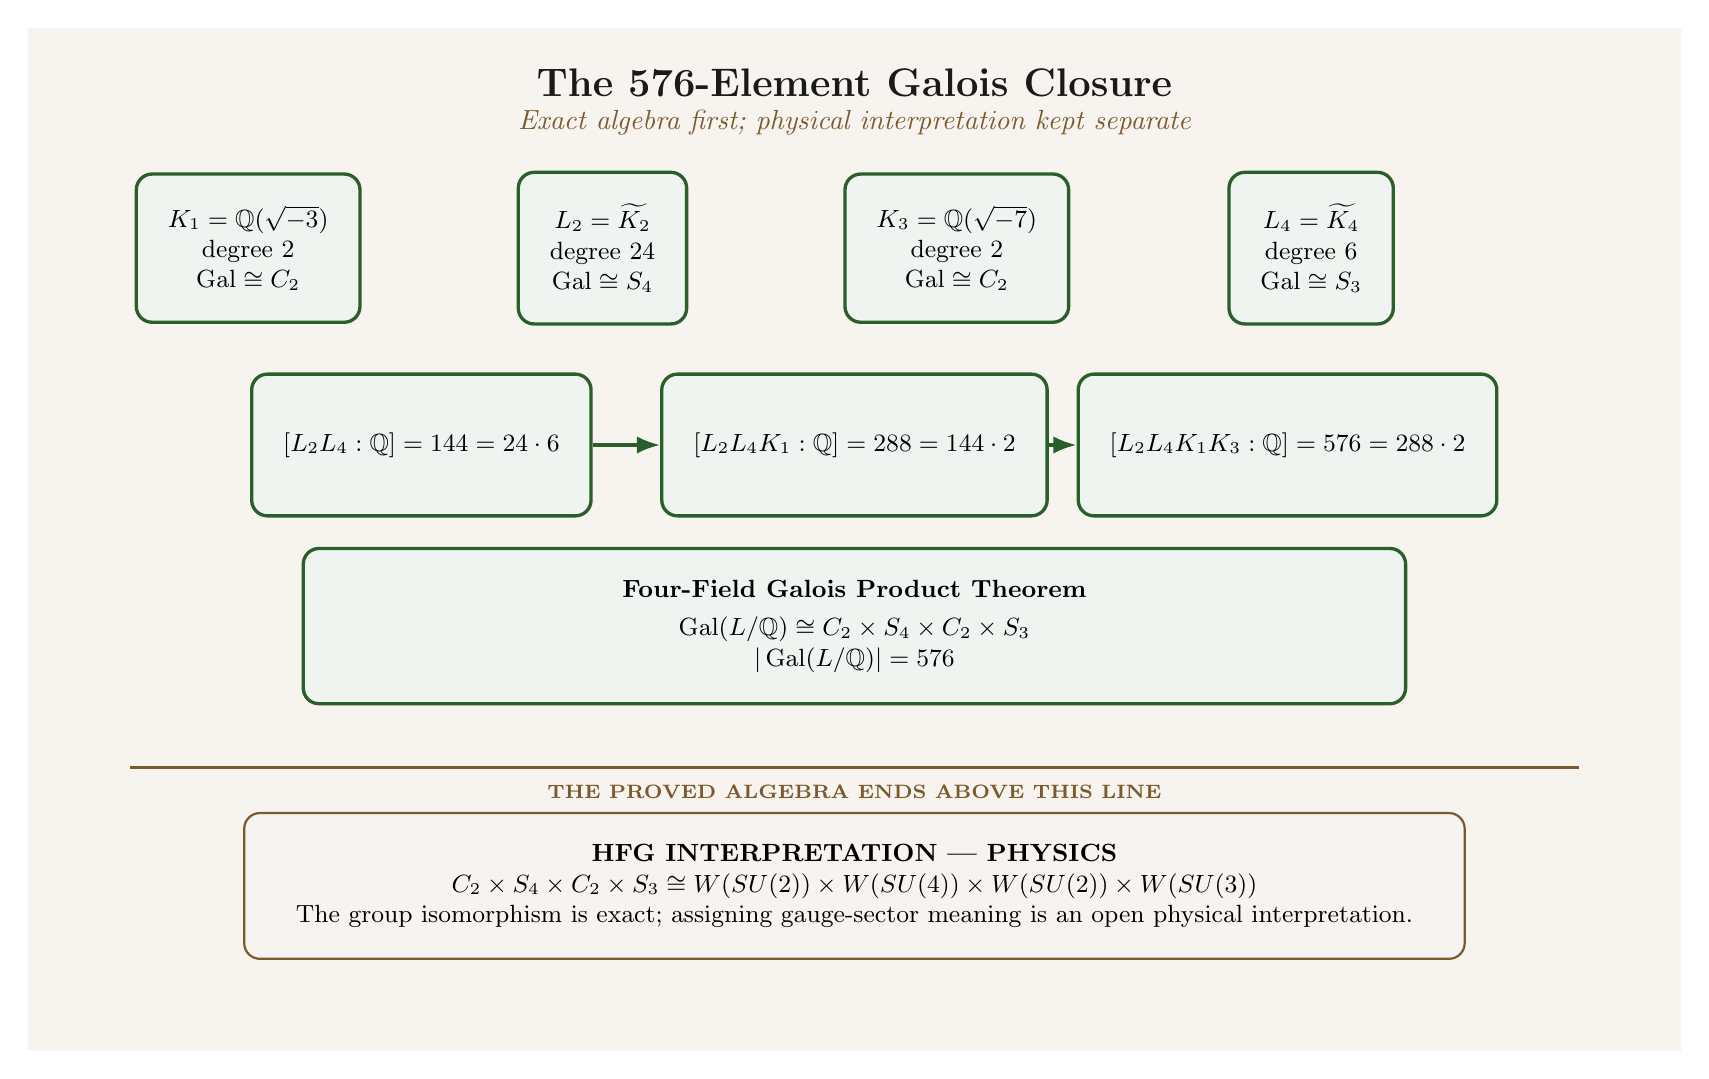
\begin{tikzpicture}[
  font=\small,
  >=Latex,
  box/.style={rounded corners=2mm, draw=proved, fill=proved!7, very thick, align=center, minimum height=18mm, inner sep=4mm},
  ibox/.style={rounded corners=2mm, draw=interp, fill=interp!7, thick, align=center, inner sep=4mm},
  arrow/.style={->, very thick, draw=proved},
]
\fill[paper] (-1,-1) rectangle (20,12);

\node[font=\Large\bfseries,text=ink] at (9.5,11.3) {The 576-Element Galois Closure};
\node[font=\itshape,text=interp] at (9.5,10.8) {Exact algebra first; physical interpretation kept separate};

\node[box] (k1) at (1.8,9.2) {$K_1=\mathbb Q(\sqrt{-3})$\\degree $2$\\$\operatorname{Gal}\cong C_2$};
\node[box] (l2) at (6.3,9.2) {$L_2=\widetilde{K_2}$\\degree $24$\\$\operatorname{Gal}\cong S_4$};
\node[box] (k3) at (10.8,9.2) {$K_3=\mathbb Q(\sqrt{-7})$\\degree $2$\\$\operatorname{Gal}\cong C_2$};
\node[box] (l4) at (15.3,9.2) {$L_4=\widetilde{K_4}$\\degree $6$\\$\operatorname{Gal}\cong S_3$};

\node[box] (d1) at (4.0,6.7) {$[L_2L_4:\mathbb Q]=144=24\cdot 6$};
\node[box] (d2) at (9.5,6.7) {$[L_2L_4K_1:\mathbb Q]=288=144\cdot 2$};
\node[box] (d3) at (15.0,6.7) {$[L_2L_4K_1K_3:\mathbb Q]=576=288\cdot 2$};

\draw[arrow] (d1) -- (d2);
\draw[arrow] (d2) -- (d3);

\node[box, minimum width=14cm] (thm) at (9.5,4.4)
{\textbf{Four-Field Galois Product Theorem}\\[1mm]
$\operatorname{Gal}(L/\mathbb Q)\cong C_2\times S_4\times C_2\times S_3$\\
$|\operatorname{Gal}(L/\mathbb Q)|=576$};

\draw[interp, line width=1.2pt] (0.3,2.6) -- (18.7,2.6);
\node[text=interp,font=\scriptsize\bfseries] at (9.5,2.3) {THE PROVED ALGEBRA ENDS ABOVE THIS LINE};

\node[ibox, minimum width=15.5cm] at (9.5,1.1)
{\textbf{HFG INTERPRETATION — PHYSICS}\\
$C_2\times S_4\times C_2\times S_3
\cong W(SU(2))\times W(SU(4))\times W(SU(2))\times W(SU(3))$\\
The group isomorphism is exact; assigning gauge-sector meaning is an open physical interpretation.};

\end{tikzpicture}
\end{document}
